\documentclass[a4j]{jsarticle}
\usepackage{graphicx}
\usepackage{listings}

\title{2024年度プログラミング\textsc{iii} 演習課題}
\author{学籍番号: 35714121 \\ 氏名: 福富隆大}
\date{2024年10月24日}

\begin{document}
\maketitle

\textbf{1 はじめに} \\

本レポートは演習課題第4回の実行結果をまとめたものである。\\

\textbf{2 課題の実行結果} \\

\textmd{(課題4-1)} \\

課題の実行結果を図1に示す。 \\

\begin{figure}[htbp]
  \centering
  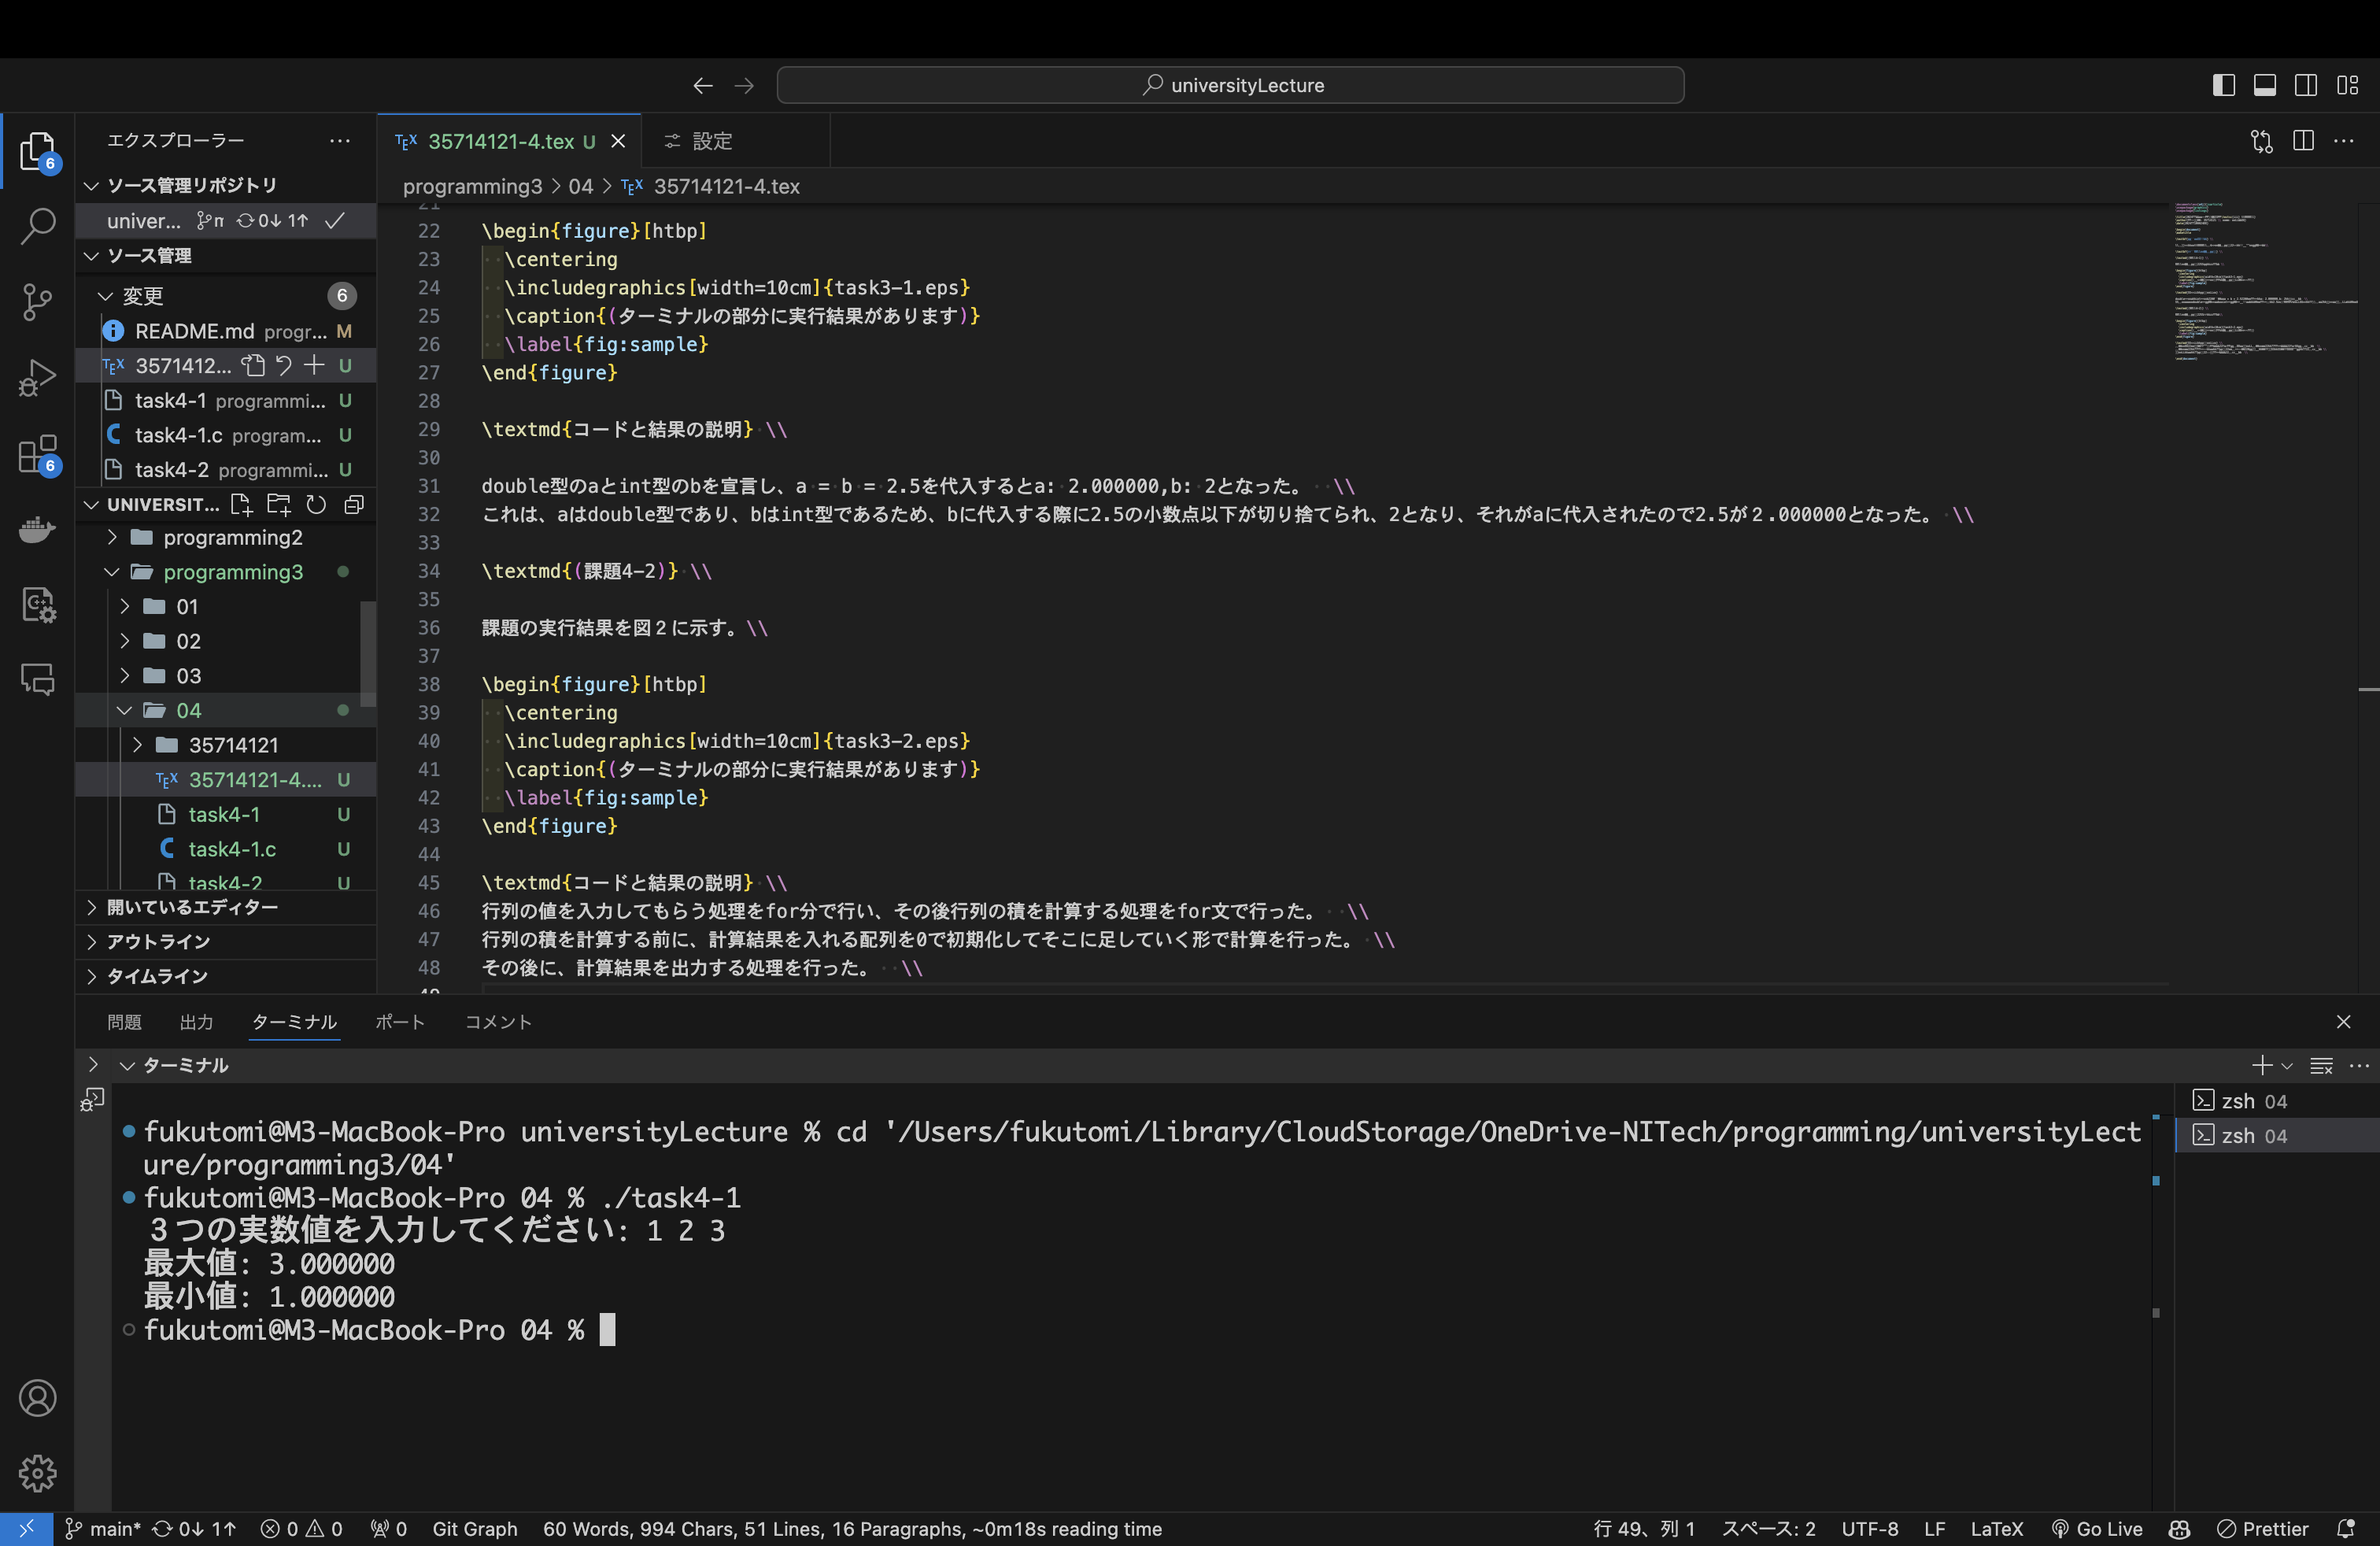
\includegraphics[width=10cm]{task4-1.eps}
  \caption{(ターミナルの部分に実行結果があります)}
  \label{fig:sample}
\end{figure}

\textmd{コードと結果の説明} \\

if文を二段階に分けて最大と最小をそれぞれ求めた。 \\
最初に、最大値を求める処理を行い、その後に最小値を求める処理を行った。 \\

\textmd{(課題4-2)} \\

課題の実行結果を図2に示す。\\

\begin{figure}[htbp]
  \centering
  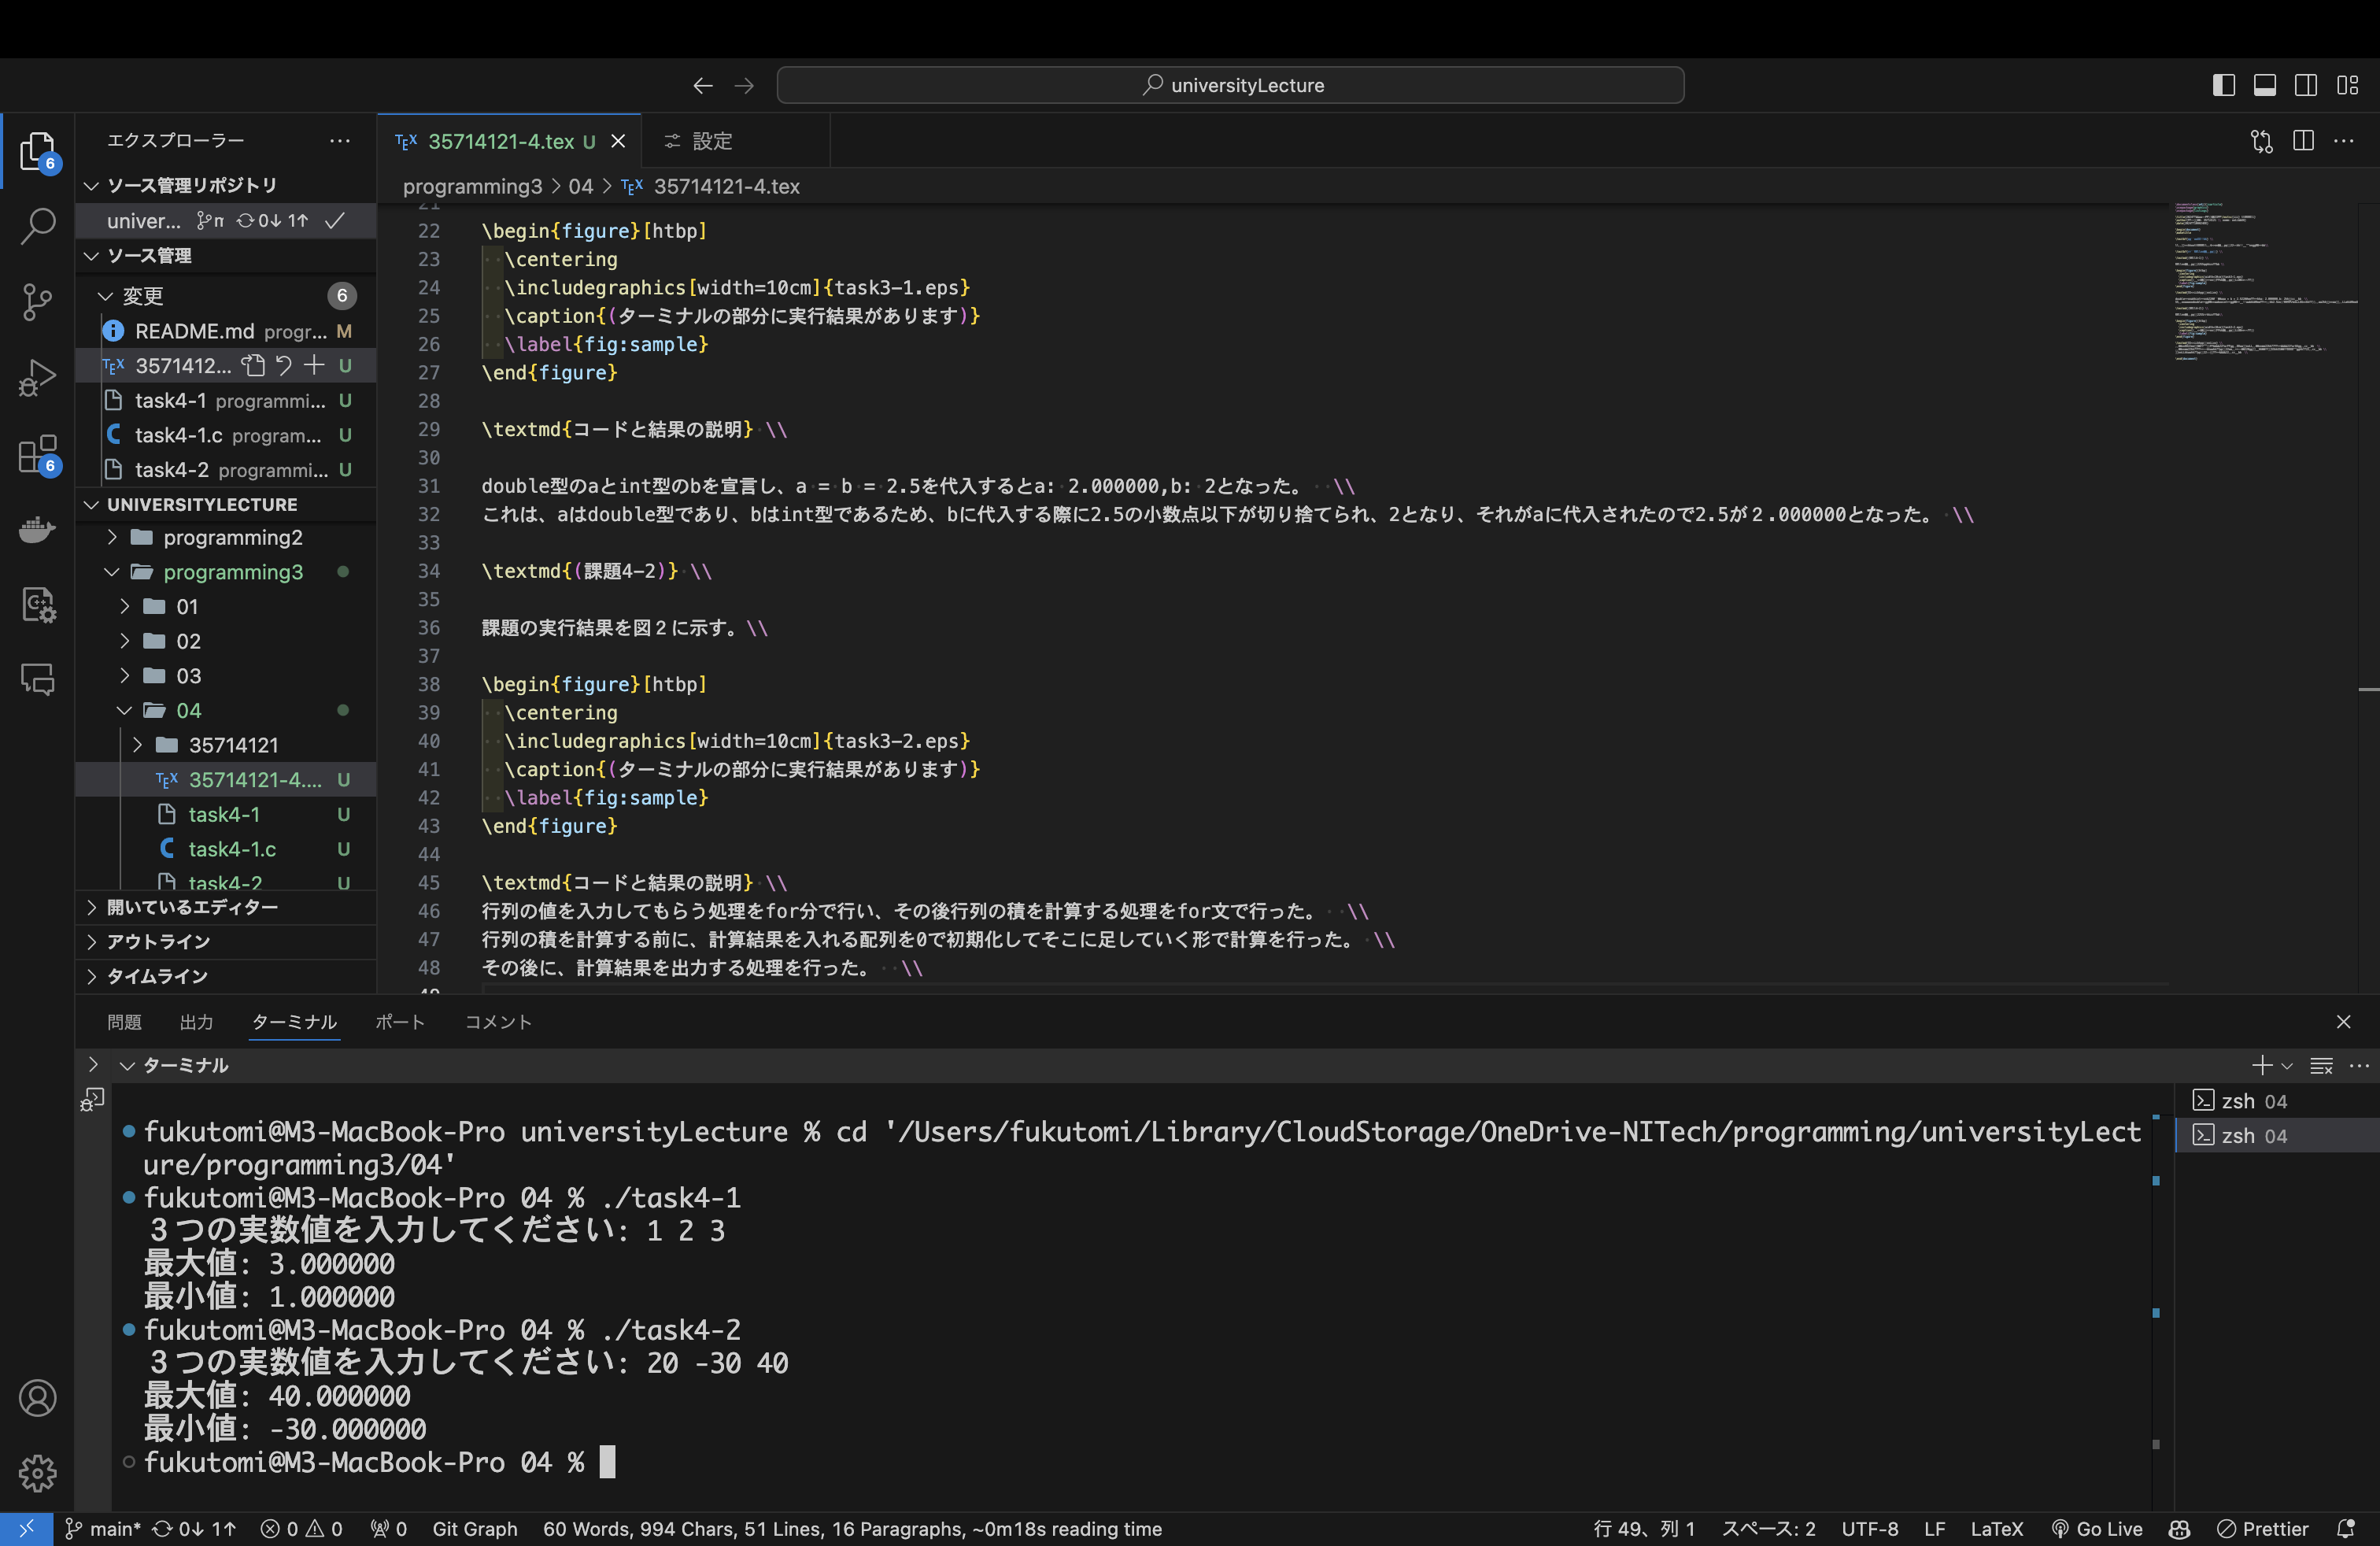
\includegraphics[width=10cm]{task4-2.eps}
  \caption{(ターミナルの部分に実行結果があります)}
  \label{fig:sample}
\end{figure}

\textmd{コードと結果の説明} \\
課題4-1で作ったif文のコードをswhich文に変更した。 \\
比較演算子の真偽によって、処理を分岐させている。 \\
しかし、swhich文はbooleanに適していないため、if文の方が適していると思う。 \\

\end{document}
